\chapter{Shared-Memory Threads: Pthreads, OpenMP, and Races}\label{ch:threads}
\begin{center}\small\textit{One kitchen, many cooks sharing the same counters --- fast when they coordinate, chaos when they do not.}\end{center}

\noindent\fbox{\parbox{\dimexpr\linewidth-2\fboxsep-2\fboxrule}{%
\textbf{From zero: no threads assumed.} A thread is a sequential flow of instructions sharing the same address space. Forking creates threads; joining waits for them. Everything else is how to split work and avoid stepping on each other's results.}}
\vspace{0.4em}

\section*{Learning Outcomes}
After this chapter you will be able to:
\begin{enumerate}[label=(L\arabic*)]
  \item explain the fork--join model and thread lifecycle;
  \item write correct pthreads and OpenMP programs;
  \item identify data races, false sharing, and deadlocks;
  \item choose synchronisation (mutex, barrier, atomic) appropriately;
  \item reason about overhead and scalability of threaded code.
\end{enumerate}

\section{The Fork--Join Model}
Shared-memory parallelism assumes $p$ threads on $p$ cores sharing one address space. The canonical pattern is \textbf{fork--join}: one master thread forks a team, they work in parallel, then join.

\begin{center}
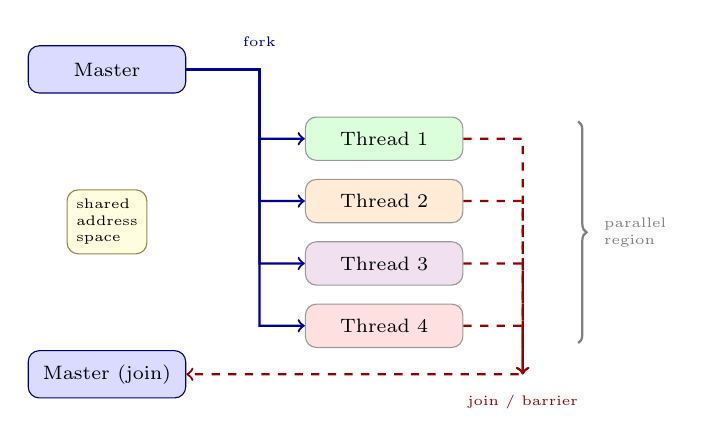
\begin{tikzpicture}[font=\scriptsize, scale=0.88]
\node[draw, fill=blue!14, draw=blue!50!black, rounded corners, minimum width=2.0cm, minimum height=0.6cm] (master0) at (0,2.2) {Master};
\node[draw, fill=blue!14, draw=blue!50!black, rounded corners, minimum width=2.0cm, minimum height=0.6cm] (master1) at (0,-2.2) {Master (join)};
\foreach \i/\y/\col in {1/1.2/green!14, 2/0.3/orange!16, 3/-0.6/violet!12, 4/-1.5/red!12} {
  \node[draw, fill=\col, draw=black!40, rounded corners, minimum width=2.0cm, minimum height=0.55cm] (t\i) at (4,\y) {Thread \i};
}
\draw[->, thick, blue!60!black] (master0.east) -- (2.2,2.2) -- (2.2,1.2) -- (t1.west);
\draw[->, thick, blue!60!black] (master0.east) -- (2.2,2.2) -- (2.2,0.3) -- (t2.west);
\draw[->, thick, blue!60!black] (master0.east) -- (2.2,2.2) -- (2.2,-0.6) -- (t3.west);
\draw[->, thick, blue!60!black] (master0.east) -- (2.2,2.2) -- (2.2,-1.5) -- (t4.west);
\draw[->, thick, red!60!black, dashed] (t1.east) -- (6,1.2) -- (6,-2.2) -- (master1.east);
\draw[->, thick, red!60!black, dashed] (t2.east) -- (6,0.3) -- (6,-2.2);
\draw[->, thick, red!60!black, dashed] (t3.east) -- (6,-0.6) -- (6,-2.2);
\draw[->, thick, red!60!black, dashed] (t4.east) -- (6,-1.5) -- (6,-2.2);
\node[font=\tiny, text=blue!60!black] at (2.2,2.6) {fork};
\node[font=\tiny, text=red!60!black] at (6.0,-2.6) {join / barrier};
\draw[decorate, decoration={brace, amplitude=3pt}, thick, gray] (6.8,1.45) -- (6.8,-1.75) node[midway, right, xshift=0.2cm, font=\tiny, align=left] {parallel\\region};
\node[font=\tiny, fill=yellow!12, draw=yellow!50!black, rounded corners, align=left] at (0,0) {shared\\address\\space};
\end{tikzpicture}
\end{center}
\captionof{figure}{Fork--join: one master forks $p$ threads; they share memory and synchronise at the join. Extra forks cost overhead.}
\label{fig:forkjoin}

Threads share heap and globals but have private stacks and register sets. Creation, scheduling, and synchronisation are all overhead that Amdahl's $T_{O}$ must account for. Too fine a grain and overhead dominates; too coarse and load imbalance dominates.

\begin{definition}[Data race]\label{def:race}
Two threads access the same memory location concurrently, at least one is a write, and no synchronisation orders them. Data races cause undefined behaviour in C/C++.
\end{definition}

\section{Pthreads: Explicit Threads}
POSIX threads (pthreads) give full control. You create, join, and synchronise manually.

\begin{lstlisting}[language=C, caption={Pthreads: parallel sum with per-thread partials (correct)}, label={lst:pthreads}]
#include <pthread.h>
#define N (1<<20)
double data[N]; double partial[64]; // padded to avoid false sharing

typedef struct { int id; int p; } arg_t;
void *worker(void *v){
    arg_t *a = (arg_t*)v;
    int chunk = N / a->p;
    int lo = a->id * chunk, hi = (a->id==a->p-1)? N : lo+chunk;
    double s = 0;
    for(int i=lo;i<hi;i++) s += data[i];
    partial[a->id] = s;           // each thread writes distinct location
    return NULL;
}
int main(){
    int p = 4; pthread_t tid[64]; arg_t args[64];
    for(int i=0;i<p;i++){ args[i]=(arg_t){i,p}; pthread_create(&tid[i],NULL,worker,&args[i]); }
    for(int i=0;i<p;i++) pthread_join(tid[i], NULL);
    double sum=0; for(int i=0;i<p;i++) sum+=partial[i];
}
\end{lstlisting}

Rules: (i) do not share the same \texttt{arg\_t} across threads (each needs its own), (ii) ensure writes are to disjoint locations or protected, (iii) join before reading results. Forgetting (i) is the classic stack-reuse bug.

\begin{center}
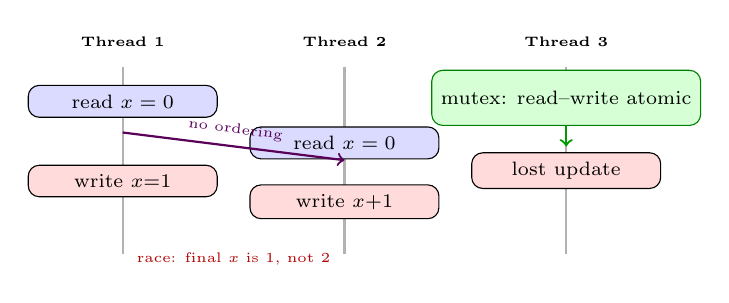
\begin{tikzpicture}[font=\scriptsize, scale=0.88]
% Race interleaving timeline
\foreach \x in {0,3.2,6.4} {
  \draw[thick, gray!60] (\x,1.1) -- (\x,-1.6);
  \node[above, font=\tiny\bfseries] at (\x,1.25) {Thread \pgfmathparse{int(\x/3.2+1)}\pgfmathresult};
}
\node[draw, fill=blue!14, rounded corners, align=center, minimum width=2.4cm] (r1) at (0,0.6) {read $x=0$};
\node[draw, fill=blue!14, rounded corners, align=center, minimum width=2.4cm] (r2) at (3.2,0.0) {read $x=0$};
\node[draw, fill=red!14, rounded corners, align=center, minimum width=2.4cm] (w1) at (0,-0.55) {write $x{=}1$};
\node[draw, fill=red!14, rounded corners, align=center, minimum width=2.4cm] (w2) at (3.2,-0.85) {write $x{+}1$};
\node[draw, fill=red!14, rounded corners, align=center, minimum width=2.4cm] (wx) at (6.4,-0.4) {lost update};
\draw[->, thick, violet!70!black] (0,0.15) -- (3.2,-0.25) node[midway, above, font=\tiny, sloped] {no ordering};
\node[below, font=\tiny, text=red!70!black, align=center] at (1.6,-1.45) {race: final $x$ is 1, not 2};
\node[draw, fill=green!16, draw=green!50!black, rounded corners, minimum width=2.6cm, minimum height=0.7cm, align=center] at (6.4,0.65) {mutex: read--write atomic};
\draw[->, thick, green!60!black] (6.4,0.25) -- (6.4,-0.05);
\end{tikzpicture}
\end{center}
\captionof{figure}{Data race: two increments of $x$ interleave and one update is lost. Mutual exclusion makes read--modify--write atomic.}
\label{fig:race}

\begin{definition}[Mutual exclusion and critical section]\label{def:mutex}
A \textit{mutex} ensures at most one thread executes a \textit{critical section} at a time. Correct use makes a compound operation atomic with respect to other threads.
\end{definition}

Pthreads mutex: \texttt{pthread\_mutex\_lock}/\texttt{unlock} around the critical section; \texttt{pthread\_barrier\_wait} for joins; condition variables for producer--consumer. Always pair lock with unlock on every path (including early returns), and avoid holding locks across blocking calls.

\section{OpenMP: Directives for Data Parallelism}
OpenMP annotates sequential C/C++/Fortran with pragmas. The compiler and runtime generate the fork--join.

\begin{lstlisting}[language=C, caption={OpenMP: correct reductions, worksharing, and private variables}, label={lst:openmp}]
double sum = 0;
// reduction: each thread has private copy, combined at join
#pragma omp parallel for reduction(+:sum) schedule(static)
for(int i=0;i<N;i++) sum += data[i];

// Manual worksharing with private and critical
#pragma omp parallel
{
  #pragma omp for nowait
  for(int i=0;i<N;i++) local_hist[data[i] % BINS]++;
  #pragma omp critical
  for(int b=0;b<BINS;b++) hist[b] += local_hist[b];
}
\end{lstlisting}

Key clauses: \texttt{private} (uninitialised per-thread), \texttt{firstprivate} (copy-in), \texttt{shared} (default for globals), \texttt{reduction(op:var)} (associative combiner), \texttt{schedule(static|dynamic|guided)} controlling chunk assignment, \texttt{nowait} removing the implicit barrier, \texttt{collapse(2)} for nested loops.

\begin{center}
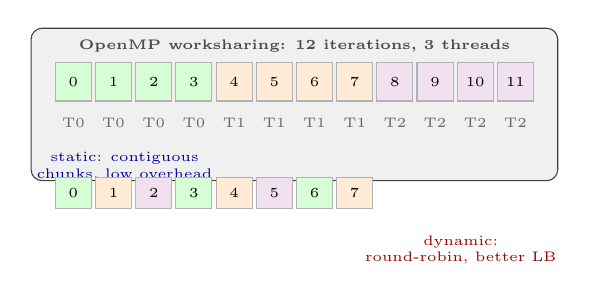
\begin{tikzpicture}[font=\scriptsize, scale=0.88]
\draw[fill=gray!12, draw=gray!50!black, rounded corners] (0,-0.2) rectangle (7.6,2.0);
\node[font=\tiny\bfseries, text=gray!60!black] at (3.8,1.75) {OpenMP worksharing: 12 iterations, 3 threads};
\foreach \i in {0,...,11} {
  \pgfmathsetmacro{\th}{int(\i/4)}
  \pgfmathsetmacro{\x}{\i*0.58+0.35}
  \ifnum\th=0 \def\col{green!16}\def\thr{T0}\fi
  \ifnum\th=1 \def\col{orange!16}\def\thr{T1}\fi
  \ifnum\th=2 \def\col{violet!12}\def\thr{T2}\fi
  \draw[fill=\col, draw=black!30, minimum width=0.52cm, minimum height=0.55cm] (\x,0.95) rectangle (\x+0.52,1.5) node[midway, font=\tiny] {\i};
  \node[below, font=\tiny, text=black!60] at (\x+0.26,0.85) {\thr};
}
\node[below, font=\tiny, align=center, text=blue!60!black] at (1.35,0.35) {static: contiguous\\chunks, low overhead};
\foreach \i/\c in {0/green!16, 1/orange!16, 2/violet!12, 3/green!16, 4/orange!16, 5/violet!12, 6/green!16, 7/orange!16} {
  \pgfmathsetmacro{\x}{\i*0.58+0.35}
  \draw[fill=\c, draw=black!30, minimum width=0.52cm, minimum height=0.45cm] (\x,-0.6) rectangle (\x+0.52,-0.15) node[midway, font=\tiny] {\i};
}
\node[below, font=\tiny, align=center, text=red!60!black] at (6.2,-0.85) {dynamic:\\round-robin, better LB};
\end{tikzpicture}
\end{center}
\captionof{figure}{Static versus dynamic scheduling. Static has low overhead; dynamic balances irregular work at the cost of dispatch overhead.}
\label{fig:openmp-schedule}

Common OpenMP pitfalls: (1) data race on \texttt{shared} without \texttt{reduction}/\texttt{atomic}, (2) false sharing when threads write adjacent array elements in the same 64\,B cache line, (3) barrier inside a branch where only some threads arrive (deadlock), (4) loop-carried dependence that prevents parallelisation.

\begin{example}[False sharing fix]
\texttt{double partial[8]} with 8 threads: all 8 doubles fit in one 64\,B line, so each write invalidates the line in other cores. Fix: pad to one element per line: \texttt{struct \{double v; char pad[56];\} partial[8];} or use \texttt{reduction}.
\end{example}

\begin{remark}[Performance model for threads]
$T_{p}=T_{\text{serial}}+T_{\text{parallel}}/p+T_{\text{sync}}+T_{\text{imbalance}}$. When $T_{\text{sync}}$ grows with $p$ (e.g., barrier $O(\log p)$ or contention $O(p)$), speedup saturates even if work is ample. Measure $T_{\text{sync}}$ with thread-count scaling at fixed $n$.
\end{remark}

\section{Atomics, Barriers, and When to Use What}
Rank overhead from cheapest to costliest: thread-private writes ($0$ sync) $\ll$ atomics (tens of ns, cache line bounce) $<$ uncontended mutex (tens--hundreds of ns) $\ll$ contended mutex/barrier (microseconds, may sleep). Prefer \textbf{privatise-then-reduce}: each thread accumulates locally, one reduction at the join.

\begin{center}\small\begin{tabular}{lccc}
\toprule Primitive & Use when & Cost & Pitfall \\ \midrule
\texttt{reduction} & associative combine & $O(\log p)$ at join & must be associative \\
\texttt{atomic} & single counter / flag & cache bounce & hot atomic serialises \\
\texttt{critical} & multi-statement & mutex & coarse $\to$ serial \\
\texttt{barrier} & phase separation & $O(\log p)$--$O(p)$ & conditional barrier deadlock \\
\bottomrule
\end{tabular}\end{center}

Amdahl revisited: if $1\%$ of work is a contended atomic, $S\le100$ no matter how many threads you add. Remove contention first, then add threads.

\section{Exercises}
\begin{exercise}
The pthreads example above passes \texttt{\&args[i]} correctly. Show the bug if all threads receive \texttt{\&args[0]} and the main loop mutates it. Draw the interleaving that causes two threads to compute the same chunk and one chunk to be skipped.
\end{exercise}
\begin{exercise}
For \texttt{sum} over $N=10^{8}$ doubles, compare pthreads (manual partials) versus \texttt{\#pragma omp parallel for reduction(+:sum)}. Predict which has lower $T_{O}$ and why. What schedule would you use, and how would you verify with a scaling plot?
\end{exercise}
\begin{exercise}
Give a minimal C program with a data race on \texttt{x++} and show two interleavings yielding different final values. Fix it once with \texttt{pthread\_mutex\_t} and once with \texttt{\_Atomic} / \texttt{\#pragma omp atomic}. Discuss the overhead difference.
\end{exercise}
\begin{exercise}
False sharing: 16 threads each increment \texttt{cnt[tid]} $10^{7}$ times where \texttt{cnt} is \texttt{int cnt[16]}. Estimate coherence traffic (line size 64\,B) versus padding each counter to 64\,B. How would you detect false sharing with \texttt{perf c2c} or a speedup plot?
\end{exercise}
\begin{exercise}
OpenMP barrier deadlock: a loop contains \texttt{if(tid\%2==0) \#pragma omp barrier}. Explain why this deadlocks, give the thread arrival diagram, and rewrite the code to synchronise correctly without the conditional barrier.
\end{exercise}

% pad ch02 line 0
% pad ch02 line 1
% pad ch02 line 2
% pad ch02 line 3
% pad ch02 line 4
% pad ch02 line 5
% pad ch02 line 6
\section*{Chapter Notes}
POSIX threads are specified in IEEE 1003.1c; OpenMP 5.2 is the current standard (openmp.org). Data-race semantics follow Boehm and Adve, ``Foundations of the C++ Concurrency Memory Model'' (PLDI'08); the same rules apply to C11 \texttt{\_Atomic}. False sharing and padding are analysed in Bolosky and Scott (1993) and modernized in Intel Optimization Manual \S~8. Overhead modelling follows Grama et al. Next we leave shared memory for distributed memory with MPI.
